\documentclass[pdf,xcolor={dvipsnames}]{beamer}
\usepackage{xcolor,soul}
% \renewcommand<>{\hl}[1]{\only#2{\beameroriginal{\hl}}{#1}}

\mode<presentation>{\usetheme{default}}
\title{Improving an Exact Solution to the \newline ($l$,$d$) Planted Motif Problem}
\author{Maria Clara Isabel Sia}

\definecolor{green}{HTML}{4CBB17}
% \AtBeginSection[]{
% 	\begin{frame}{}\tableofcontents[currentsection]\end{frame}
% }

\begin{document}
\begin{frame}\titlepage\end{frame}

\section{Introduction}
	\begin{frame}{Introduction}{DNA motif finding}
		\begin{itemize}
			\item {\usebeamercolor[fg]{frametitle}motifs} are repeated sub-sequences in DNA that have some biological significance\newline
			\item {\usebeamercolor[fg]{frametitle}DNA motif finding} searches for motifs over a set of DNA sequences, allowing for mismatches due to mutation\newline
			\item known as a difficult problem in computational biology and CS (proven {\usebeamercolor[fg]{frametitle}NP-complete})\newline
		\end{itemize}
		\end{frame}

	\subsection{The ($l$,$d$) planted motif problem}
	\begin{frame}{Introduction}{The ($l$,$d$) planted motif problem}
		{
		\centering
		\emph{Find a motif of length $l$=8 across these 5 DNA sequences,}\\
		\emph{each containing the motif with at most $d$=2 mismatches.}\\
		\ \\
		% ($l$, $d$) = (8, 2)\\
		\small
		% \ \\
		$S_1$\ \ \  \texttt{at{\color{blue}c{ac}tcgtt}ctcctctaatgtgtaaagacgtactaccgacctta}\\
		$S_2$\ \ \  \texttt{acgccgaccggtc{\color{blue}c{g}atc{c}tt}gtatagctcctaacgggcatcagc}\\
		$S_3$\ \ \  \texttt{tcctgactgcatcgcgatctcggtagtttcctgt{\color{blue}{t}catc{a}tt}ttt}\\
		$S_4$\ \ \  \texttt{ggccctca{\color{blue}{g}catcgt{g}}cgtcctgctaacacattcccatgcagctt}\\
		$S_5$\ \ \  \texttt{tgaaaagaatttacggtaaaggatccacatc{\color{blue}c{a}atcgt{g}}tgaaag}\\ 
		\ \\
		\emph{Planted motif: }\texttt{\color{blue}ccatcgtt}\\
		\ \\
		}

		\end{frame}

	\begin{frame}{Introduction}{Solutions to the ($l$,$d$) planted motif problem)}
		There are two types of methods used by motif search algorithms:\\ \ \\
		\begin{itemize}
		\item {\usebeamercolor[fg]{frametitle} heuristic methods} (ex. probabilistic sampling, projection)
		perform an iterative local search which is efficient, but not guaranteed to find all motifs
		\\ \ \\
		\item {\usebeamercolor[fg]{frametitle} exact methods} (ex. combinatorial search, tree pruning)
		perform an exhaustive search which will {find all possible motifs, at the cost of time/space efficiency}
		\end{itemize}
		\end{frame}

	\subsection{$l$-mers, Hamming distances, and $d$-neighborhoods}
	\begin{frame}{Introduction}{$l$-mers, Hamming distances, and $d$-neighborhoods}
		\begin{itemize}
		\setbeamercovered{transparent=25}
		\item<1,2>{\alt<2>{\usebeamercolor[fg]{frametitle}}{} $l$-mer}
			\only<2>{ \newline- sequence of length $l$\\
				\begin{center}
				{\small
				$S_1$\ =\ \texttt{at{\color{red}c{ac}tcgtt}ctcctctaatgtgtaaagacgtactaccgacctta}\\ \ \\
				}
				\end{center}
			}
		\item<1,3> {\alt<3>{\usebeamercolor[fg]{frametitle}}{} Hamming distance $d_H$}
			\only<3>{ \\- number of mismatches between $l$-mers $x_1$ and $x_2$\\
				\begin{columns}
					\begin{column}{0.1\textwidth}\end{column}
					\begin{column}{0.4\textwidth}
					\begin{center} {
						$x_1$ = \texttt{c{\color{red}g}atc{\color{red}c}tt}\ \ \\
						$x_2$ = \texttt{c{\color{red}c}atc{\color{red} g}tt}\ \ \\
					}\end{center}
					\end{column}
					\begin{column}{0.5\textwidth}
					% \begin{center} {
						$d_H(x_1,x_2) = 2$\ \ \\
					% }\end{center}
					\end{column}
				\end{columns}
				\ \\\ \\
			}
		\item<1,4>{\alt<4>{\usebeamercolor[fg]{frametitle}}{} $d$-neighbor}
			\only<4>{ \\- two $l$-mers $x$ and $x'$ are $d$-neighbors if $d_H(x,x') \leq d$\\\ \\
				{\footnotesize 
					$N$(\texttt{ccatcgtt}, 2)\ \ \ {\color{Gray} $\rightarrow$ $d$-neighborhood of \texttt{ccatcgtt}, d=2}\\
					\hspace*{0.055\textwidth}=  \{ \texttt{ccatcgtt}, \newline
					\texttt{
						\hspace*{0.1\textwidth}
						{\color{red}a}catcgtt,{\color{red}g}catcgtt,{\color{red}t}catcgtt,%
						c{\color{red}a}atcgtt,c{\color{red}g}atcgtt,c{\color{red}t}atcgtt,
					}	
					\hspace*{0.12\textwidth}...{\color{Gray} all $l$-mers with 1 mismatch}\newline
					\texttt{
						\hspace*{0.1\textwidth}
						{\color{red}a}{\color{red}a}atcgtt,%
						{\color{red}a}{\color{red}g}atcgtt,%
						{\color{red}a}{\color{red}t}atcgtt,%
						{\color{red}g}{\color{red}a}atcgtt,%
						{\color{red}g}{\color{red}g}atcgtt,%
						{\color{red}g}{\color{red}t}atcgtt,
						\hspace*{0.1\textwidth}
						{\color{red}t}{\color{red}a}atcgtt,%
						{\color{red}t}{\color{red}g}atcgtt,%
						{\color{red}t}{\color{red}t}atcgtt,%
						{\color{red}a}c{\color{red}c}tcgtt,%
						{\color{red}a}c{\color{red}g}tcgtt,%
						{\color{red}a}c{\color{red}t}tcgtt,					
				 	}
				 	\hspace*{0.12\textwidth}...{\color{Gray} all $l$-mers with 2 mismatches}\newline
				 	\hspace*{0.095\textwidth}{\footnotesize\}}
			 	}
				% \newline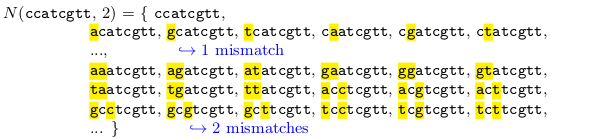
\includegraphics[width=10.5cm]{img/concepts_N(x,d)}	
			}
		% \item<1,5>{\alt<5>{\usebeamercolor[fg]{frametitle}}{} $d$-neighborhood $\mathcal{N}(S,d)$ of sequence $S$}
		% 	\only<5>{ \newline- set of all $d$-neighbors of all $l$-mers in $S$\\
		% 	{\small\ \\
		% 	$S$ = \texttt{{\color{blue}a}{\color{red}c}gccgattacatccgatccttgtatagctcctaacg{\color{blue}g}gcatcac}\\
		% 	\footnotesize
		% 	\ \\
		% 	\hspace*{-0.05\textwidth}
		% 	$\mathcal{N}(S, 2)$ = 
		% 		$N$(\texttt{\color{blue} a}cgccgat, 2) $\cup$ 
		% 		$N$(\texttt{\color{red} c}gccgatt, 2) $\cup\ ...\ \cup$
		% 		$N$(\texttt{\color{blue} g}gcatcac, 2)\\
		% 	}
		% 	% \hspace*{0.05\textwidth} {\color{blue} $\hookrightarrow$ union of $d$-neighborhoods of $l$-mers in $S$}
		% 	% \newline\newline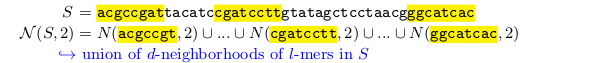
\includegraphics[width=11.0cm]{img/concepts_N(S,d)}		
		% }
		\end{itemize}
		\end{frame}

\section{EMS-GT}
	\begin{frame}{EMS-GT}{Nabos, 2014}
		\begin{itemize}
		\item an exact motif search (EMS) algorithm based on the candidate generate-and-test (GT) principle\newline
		\item solves any ($l$,$d$) planted motif problem instance, $l \leq 17$ \newline
		\item operates on a bit-based representation of the search space
		\end{itemize}
		\end{frame}

	\subsection{Generate-and-test approach}
	\begin{frame}{EMS-GT}{Generate-and-test approach}
		% The EMS-GT algorithm proceeds in two main steps:\newline
		\only<1>{
			EMS-GT proceeds in two steps:\newline
			\begin{enumerate}
			\item % Generate candidate motifs\newline
			{\usebeamercolor[fg]{frametitle}Generate the set $C$ of candidate motifs}: find
			the common $d$-neighbors of the first $n'$ sequences $S_1,S_2,...,S_{n'}$.\newline\newline
			% as the intersection of the $d$-neighborhoods of the first $n'$ sequences $S_1,S_2,...,S_{n'}$.\newline\newline
			\hspace*{14pt} {$C = \mathcal{N}(S_1,d) \cap \mathcal{N}(S_2,d) \cap ... \cap \mathcal{N}(S_{n'},d),
			\ \ \ \ n' \leq n $\newline}

			% . Every $l$-mer in the resulting set $C$ is a candidate motif.\newline
			\item % Test candidates\newline
			{\usebeamercolor[fg]{frametitle}Test every candidate $c \in C$}: if a $d$-neighbor of $c$ appears in each of the remaining sequences $S_{n'+1},S_{n'+2},...S_n$, accept $c$ as a motif.
			\end{enumerate}
		}

		 \only<2>{
		 	\bigskip\bigskip
		 	($l$,$d$) = (8,2)\newline\newline\newline
		 	\footnotesize
			$S_1$\ \ \  \texttt{at{c{ac}tcgtt}ctcctctaatgtgtaaagacgtactaccgacctta}\newline\newline\newline
			$S_2$\ \ \  \texttt{acgccgaccggtc{c{g}atc{c}tt}gtatagctcctaacgggcatcagc}\newline\newline\newline
			$S_3$\ \ \  \texttt{tcctgactgcatcgcgatctcggtagtttcctgt{{t}catc{a}tt}ttt}\newline\newline\newline

			$S_4$\ \ \  \texttt{ggccctca{{g}catcgt{g}}cgtcctgctaacacattcccatgcagctt}\newline\newline\newline
			$S_5$\ \ \  \texttt{tgaaaagaatttacggtaaaggatccacatc{c{a}atcgt{g}}tgaaag}\newline\newline\newline
		% 	includegraphics[width=10.0]{ems-gt_demo}
		 }
		\end{frame}

	\subsection{Bit-based representation of the search space}
	\begin{frame}{EMS-GT}{Bit-based representation of the search space}
		\begin{itemize}
		{
			\item The search space contains all $4^l$ possible $l$-mers that can be formed with
			$\Sigma$ = \{\texttt{a}, \texttt{c}, \texttt{g}, \texttt{t}\}. \\\ \\
			\item To represent sets in this space, EMS-GT assigns each of the $4^l$ $l$-mers a bit flag,
			which is 1 if the $l$-mer is a member of the set, 0 otherwise.\\\ \\
			\item For efficiency, EMS-GT stores the $4^l$ bits as $\frac{4^l}{32}$ 32-bit integers.
		}
		\end{itemize}
		\end{frame}

	\subsection{Bit-based representation of the search space}
	\begin{frame}{EMS-GT}{Bit-based representation of the search space}
		\begin{itemize}
			\item $N$(\ \texttt{acgt}, 1\ ): $4^l$ = 256, $\frac{4^l}{32}$ = 8
		\end{itemize}\ \\\ \\
		
		{ \centering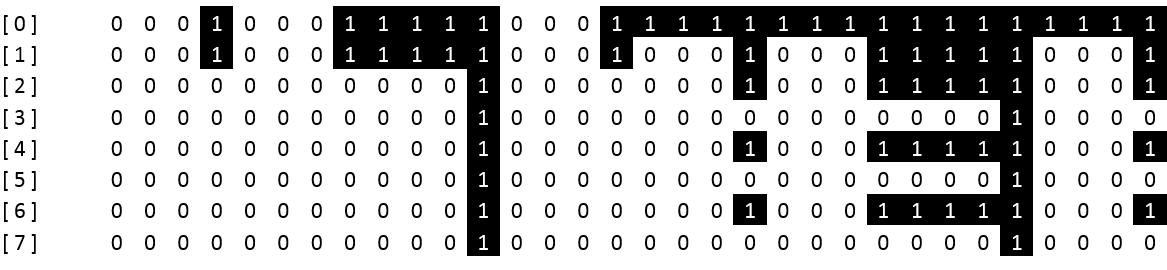
\includegraphics[width=\textwidth]{img/acgt_labeled.png}\\ }
		\ \\
		\begin{itemize}
			\item EMS-GT generates a neighborhood bit-array by generating each individual neighbor, then finding and setting its bit flag.
		\end{itemize}
		\end{frame}

	% \begin{frame}{EMS-GT}{Bit-based representation of the search space}
		% \begin{itemize}
		% \setbeamercovered{transparent=25}
		% \item<1,2> {\alt<2>{\usebeamercolor[fg]{frametitle}}{} $l$-mer enumeration scheme}
		% 	\only<2>{
		% 	\newline EMS-GT maps an $l$-mer to a $2l$-bit binary number by replacing each
		% 	character with two bits (\texttt{a=00}, \texttt{c=01}, \texttt{g=10}, \texttt{t=11}).\newline\newline
		% 	% This scheme enumerates $l$-mers in alphabetical order.
		% 		{
		% 		\scriptsize
		% 		{\LARGE\texttt{aaaaa}}\ \ {\LARGE\texttt{aaaa{\color{blue}c}}}\ \ {\LARGE\texttt{aaaa{\color{blue}g}}} ...,\ %
		% 		{\LARGE\texttt{{\color{blue}t}a{\color{blue}c}{g}{\color{blue}t}}}\ \ {\LARGE\texttt{{\color{blue}t}a{\color{blue}c}t{\color{blue}a}}} ...
		% 		\newline
		% 		\texttt{0000000000},\ \ \texttt{00000000{\color{blue}01}},\ \ \texttt{00000000{\color{blue}10}}, ...,
		% 		\texttt{{\color{blue}11}00{\color{blue}01}{10}{\color{blue}11}},\ \ \texttt{{\color{blue}11}00{\color{blue}01}11{\color{blue}00}}, ...	\newline
		% 			{
		% 			\normalsize
		% 			\color{blue} \hspace*{0.05\textwidth}
		% 			$\hookrightarrow$ 0 \hspace*{0.07\textwidth}
		% 			$\hookrightarrow$ 1 \hspace*{0.07\textwidth}
		% 			$\hookrightarrow$ 2 \hspace*{0.08\textwidth}
		% 			$\hookrightarrow$ 795 \hspace*{0.04\textwidth}
		% 			$\hookrightarrow$ 796
		% 			\newline
		% 			}
		% 		}
		% 	}
		% \item<1,3> {\alt<3>{\usebeamercolor[fg]{frametitle}}{} Bit-based representation of sets}
		% 	\only<3>{
		% 	\newline 
		% 	The motif search space includes all $4^l$ $l$-mers that can be formed with $\Sigma$ = \{\texttt{a}, \texttt{c}, \texttt{g}, \texttt{t}\}. To represent sets in this space, EMS-GT assigns each $l$-mer a bit flag: % $set to 1 if the $l$-mer is a member of the set, 0 otherwise.
		% 	\begin{equation*}
		% 		Flags[\ {\color{blue}795}\ ] = \left\{
		% 		\begin{array}{rl}
		% 			1 & \text{if } \texttt{\color{blue}tacgt} \text{ is a member of the set}, \\
		% 			0 & \text{otherwise.}%\text{if } dH(x,x') > d.
		% 		\end{array} \right.
		% 		\end{equation*}			
		% 	}
		% \item<1,4> {\alt<4>{\usebeamercolor[fg]{frametitle}}{} Bit-array compression}
		% 	\only<4>{
		% 	\\ EMS-GT stores $4^l$ bit flags as an array of $\frac{4^l}{32}$ 32-bit integers.\\
		% 	\footnotesize\ \\
		% 	Ex. the flag for \texttt{\color{blue}tacgt} is in int index ${\color{blue}\frac{795}{32}} = {24}$, at bit ${\footnotesize({\color{blue}795\ mod\ 32})} = {27}$.\\
		% 	\ \\
		% 	\hspace*{0.3\textwidth} {\tiny\color{blue}27}\\
		% 	{\centering
		% 		{\tiny23}\ \ 			  {\color{Gray}0000{\color{black}0}011100001000100100000110011}\\
		% 		{\tiny\color{blue}24}\ \  {\color{Gray}001{\color{black}1{\color{blue}0}1}11100000000011100000011100}\\
		% 		{\tiny25}\ \ 			  {\color{Gray}1111{\color{black}1}001011001000011111100000011}\\
		% 	\ \\
		% 	}
		% 	}
		% \item<1,5> {\alt<5>{\usebeamercolor[fg]{frametitle}}{} Recursive neighborhood generation}
		% 	\only<5>{\newline To generate a $d$-neighborhood, EMS-GT recursively generates each $d$-neighbor, then finds and sets its bit flag.\\ \ \\
		% 	Generating a $d$-neighbor changes up to $d$ characters in $x$, with 3 alternatives per change (ex. \texttt{c} $\rightarrow$ \texttt{a}, \texttt{g} or \texttt{t}); thus,
		% 	\begin{equation*}\text{$l$-mer $x$ will have}\ \ \ \ 
		% 	{\color{blue}
		% 	\sum_{i=0}^d \binom{l}{i} 3^{i}}\ \ \ \ \text{possible $d$-neighbors.\ \  }\end{equation*} 
		% 	\ \\			
		% 	}
		% \end{itemize}
		% \end{frame}

	\begin{frame}{EMS-GT}{Bit-based representation of the search space}
		{\centering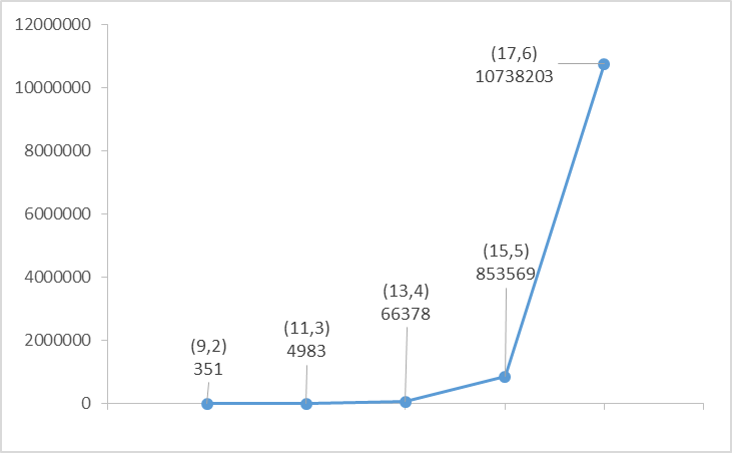
\includegraphics[width=0.8\textwidth]{img/nbrhd_growth}\\}
		\begin{itemize}
		\item $l$-mer neighborhoods grow very quickly with ($l$,$d$), meaning that EMS-GT must spend more time locating and setting bits.\\
		\end{itemize}
		\end{frame}

\section{Research objectives}
	\begin{frame}{Research objectives}{Improving EMS-GT}
		The main objectives of this research are:\\ \ \\
		\begin{enumerate}
		\item To {\usebeamercolor[fg]{frametitle}develop a speedup technique} for EMS-GT that takes advantage of distance-related patterns in the search space;\\ \ \\
		\item To {\usebeamercolor[fg]{frametitle}evaluate} the speedup technique with regard to {\usebeamercolor[fg]{frametitle}improvement in runtime}; and\\ \ \\
		\item To {\usebeamercolor[fg]{frametitle}evaluate} the improved version of the EMS-GT algorithm\\ {\usebeamercolor[fg]{frametitle}against state-of-the-art} motif search algorithms.
		\end{enumerate}
		\end{frame}
	
	% \subsection{Work summary}
	% \begin{frame}{Methods}{Work summary}
	% 	To fulfill these objectives, we:\\ \ \\
	% 	\begin{itemize}
	% 	\item %\emph{Developing an EMS-GT speedup technique}\newline
	% 	{\usebeamercolor[fg]{frametitle} investigated repeating block patterns} in EMS-GT's bit-based representation of an $l$-mer neighborhood;\\ \ \\

	% 	\item {\usebeamercolor[fg]{frametitle} designed a more efficient bit-setting procedure} that sets bits according to these block patterns; and\\ \ \\
		
	% 	\item {\usebeamercolor[fg]{frametitle} measured EMS-GT's performance} on synthetic data for ``challenging'' ($l$,$d$): (9,2), (11,3), (13,4), (15,5) and (17,6).
	% 	% \begin{itemize}
	% 	% \item synthetic dataset: $n$=20 randomly-generated DNA sequences of length $L$=600, with an ($l$,$d$) motif planted in each sequence
	% 	% \end{itemize}
	% 	\end{itemize}
	% 	\end{frame}

\section{Speedup technique}
	\begin{frame}{Speedup technique}{Key observation}
		\begin{itemize}
		\item<1-> If a bit-array $N_x$ representing the neighborhood of $l$-mer $x$
		\\ is partitioned into blocks of $4^k$ bits each,\\\ \\
		\end{itemize}
		\uncover<2->{\centering
			Ex.\ \ \large $N$(\ \texttt{acgtacgtacgt}, 5\ ), $k$ = 5\\
			\normalsize block size = $4^5 = 1024 = 32 \times 32$\\\ \\
		}
		\begin{itemize}
		\item<3-> the $4^k$ $l$-mers represented in a block will all begin with the same {\usebeamercolor[fg]{frametitle}prefix} (first $l-k$ characters), and will differ only in the {\usebeamercolor[fg]{frametitle}$k$-suffix} (last $k$ characters);\\\ \\
		\item<4-> {\usebeamercolor[fg]{frametitle}each block conforms to one of ($k + 2$) patterns.}\\\ \\
		\end{itemize}
		\ \\
	\end{frame}

	\begin{frame}{Speedup technique}{Block patterns in the $d$-neighborhood of \texttt{acgtacgtacgt}, $d$=5, $k$=5}
		\begin{columns}
			\begin{column}{0.33\textwidth}
				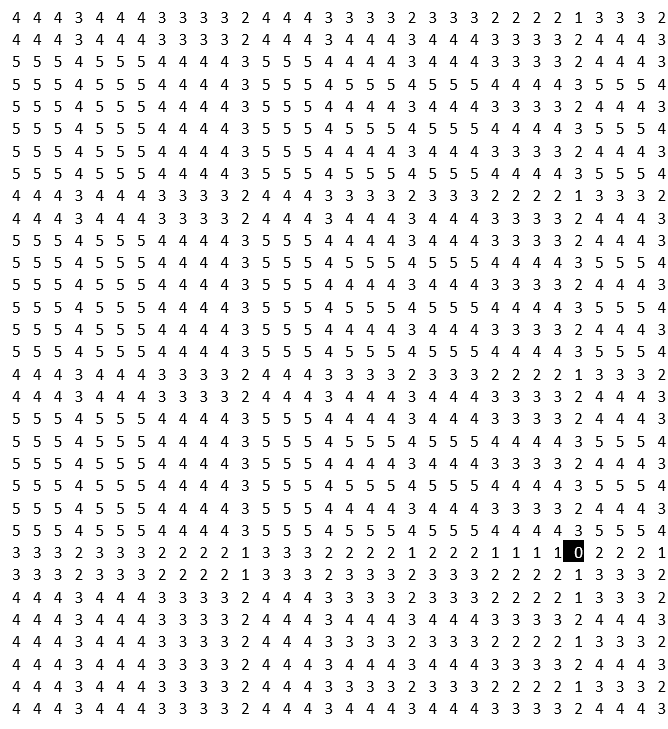
\includegraphics[width=0.9\textwidth]{img/0.png}\\\ \\
				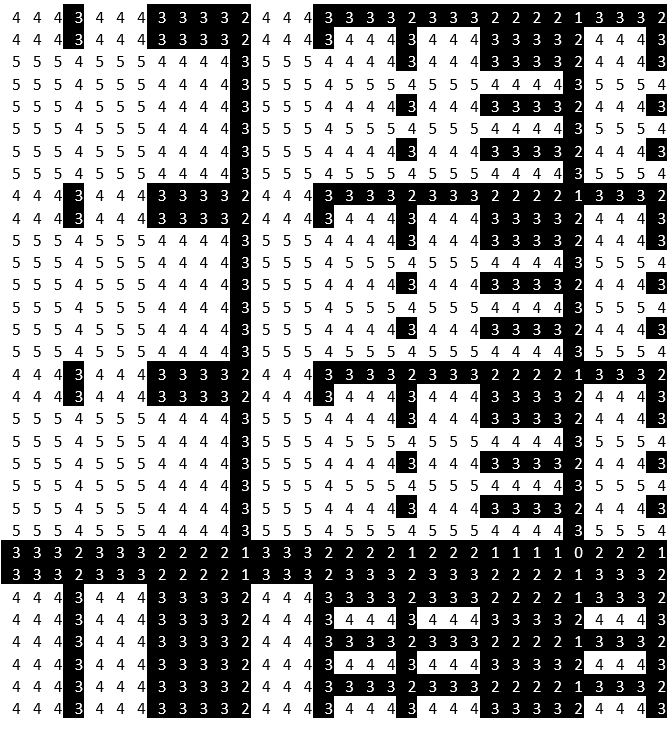
\includegraphics[width=0.9\textwidth]{img/3.png}
			\end{column}
			\begin{column}{0.33\textwidth}
				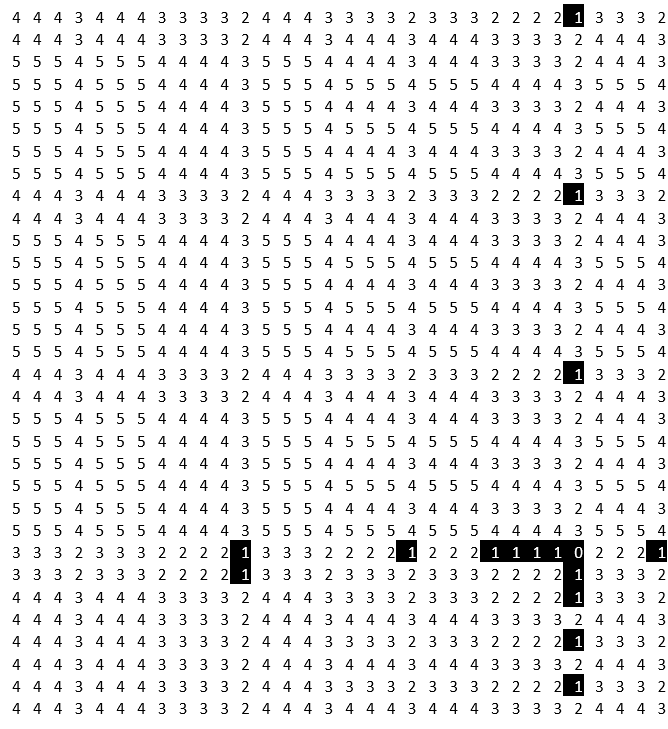
\includegraphics[width=0.9\textwidth]{img/1.png}\\\ \\
				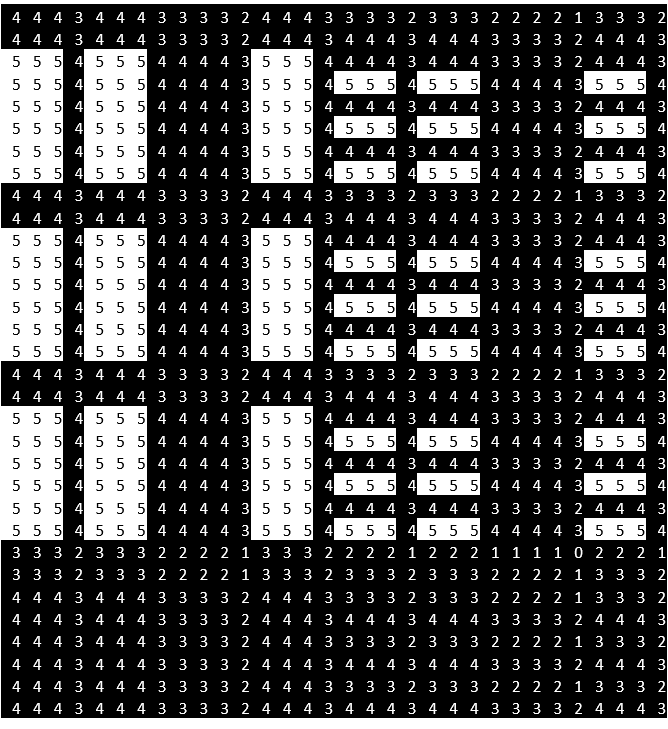
\includegraphics[width=0.9\textwidth]{img/4.png}
			\end{column}
			\begin{column}{0.33\textwidth}
				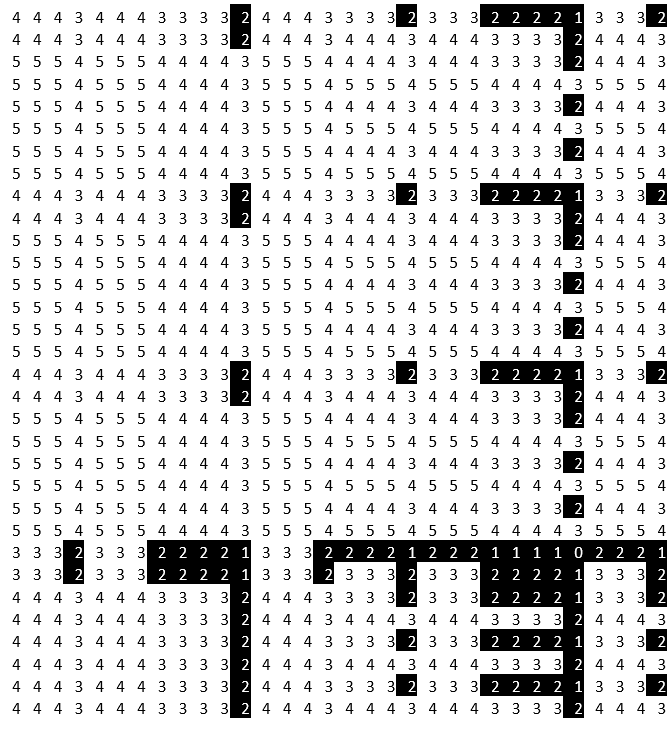
\includegraphics[width=0.9\textwidth]{img/2.png}\\\ \\
				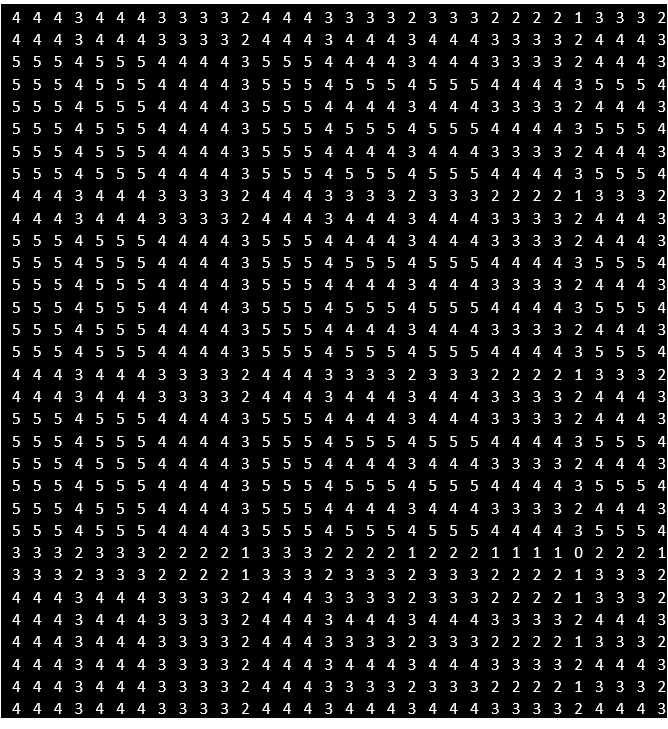
\includegraphics[width=0.9\textwidth]{img/5.png}
			\end{column}
		\end{columns}
	\end{frame}

	\begin{frame}{Speedup technique}{Key observation}
		\begin{itemize}
			\item In a $d$-neighbor of $x$, the $d$ allowable mismatches from $x$ are distributed between the prefix and the $k$-suffix.\\\ \\
			\texttt{\large\centering
				acgtacg tacgt\\
				acg{\color{red}a}a{\color{red}aa} t{\color{red}c}cg{\color{red}a}\\\ \\
			}
			\item If a {\usebeamercolor[fg]{frametitle}block's prefix already has $p$ mismatches} from $x$'s prefix, then within that block, {\usebeamercolor[fg]{frametitle}any neighbor must have a suffix with at most $d-p$ mismatches} from $x$'s suffix.
		\end{itemize}

	\end{frame}

	\begin{frame} %% THE COLORING-IN SEQUENCE
			\begin{columns}[c]
			\begin{column}{2.0cm}
			\begin{flushright}{aaaaa $\rightarrow$}\end{flushright}
			\ \\\ \\\ \\\ \\\ \\\ \\\ \\\ \\\ \\\ \\
			\ \\\ \\\ \\\ \\\ \\\ \\\ \\\ \\\ \\
			\end{column}
			\begin{column}{8.0cm}
			\only<1>{\centering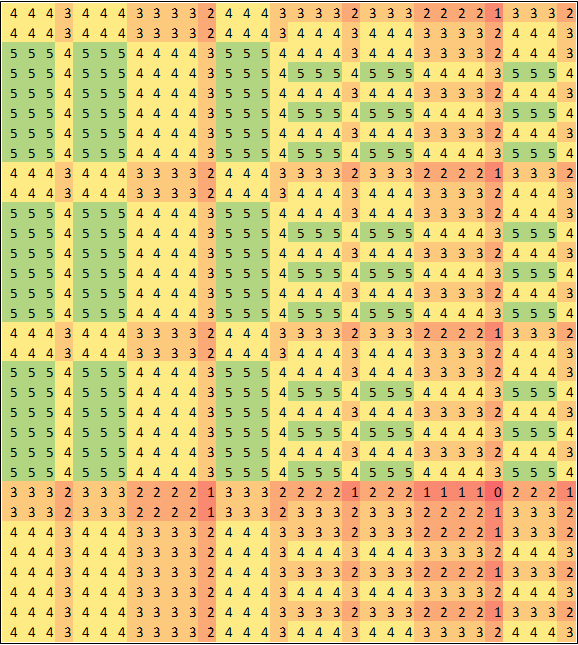
\includegraphics[width=8.0cm, height=8.6cm]{img/D(tacgt)}\\}
			\only<2>{\centering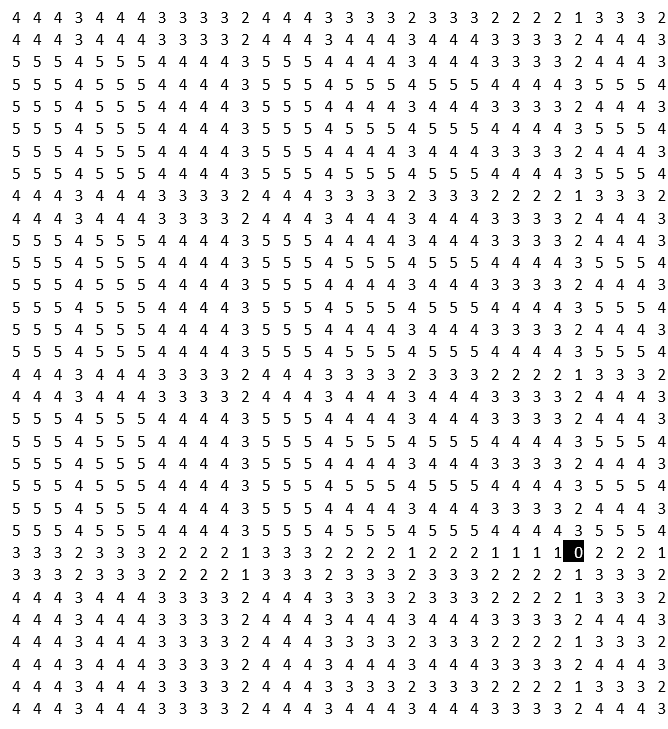
\includegraphics[width=8.0cm]{img/0}\\}
			\only<3>{\centering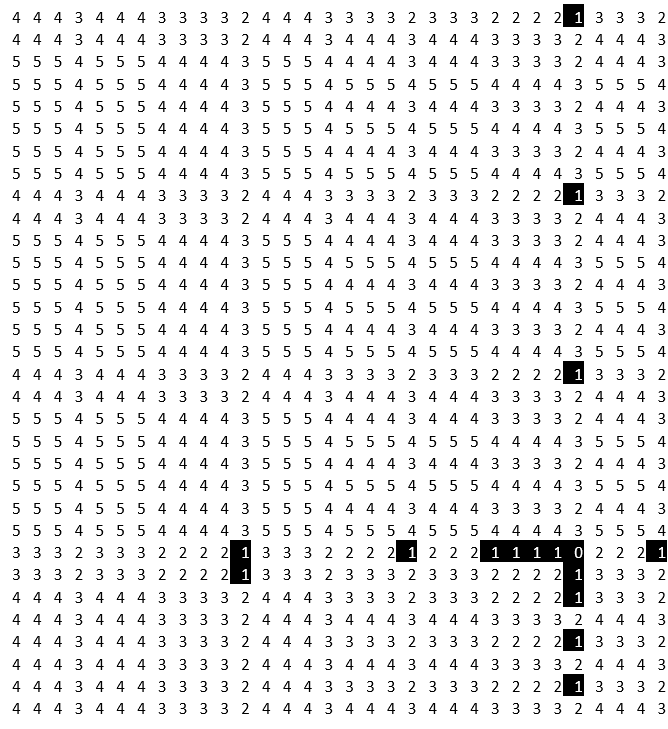
\includegraphics[width=8.0cm]{img/1}\\}
			\only<4>{\centering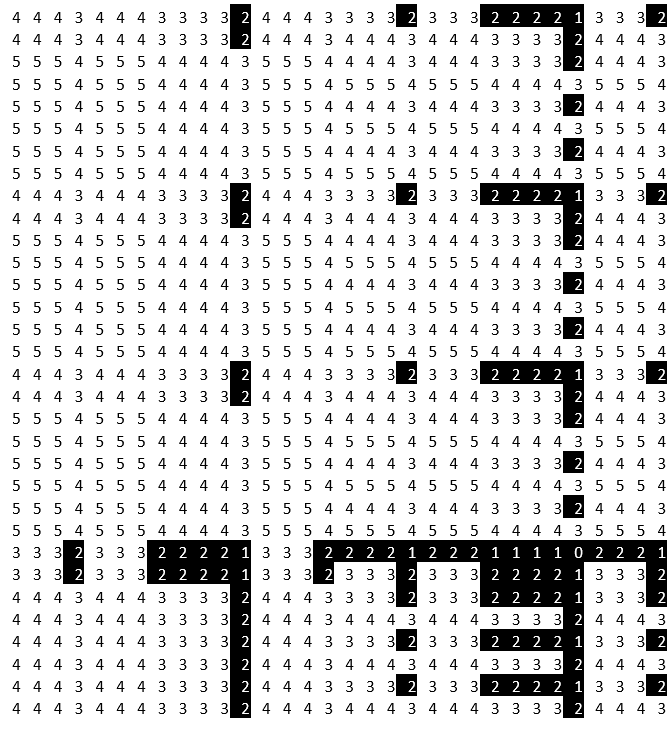
\includegraphics[width=8.0cm]{img/2}\\}
			\only<5>{\centering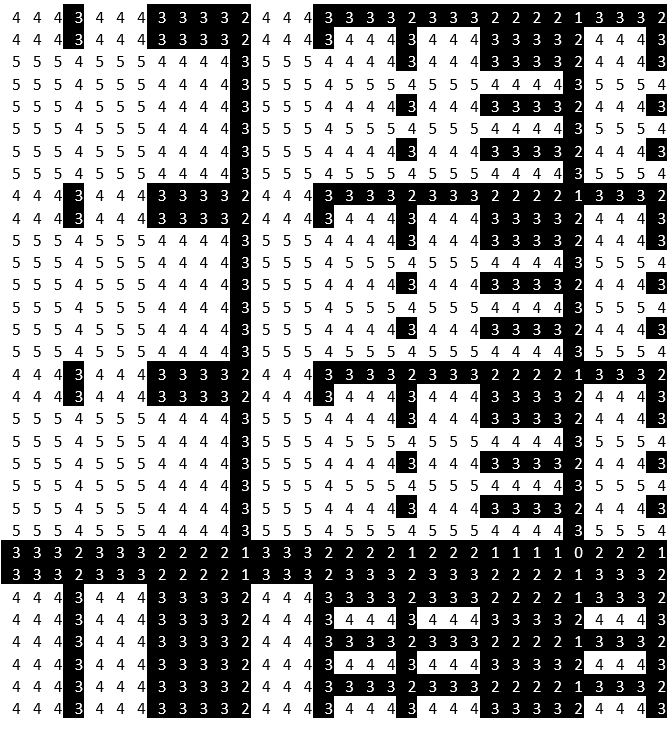
\includegraphics[width=8.0cm]{img/3}\\}
			\only<6>{\centering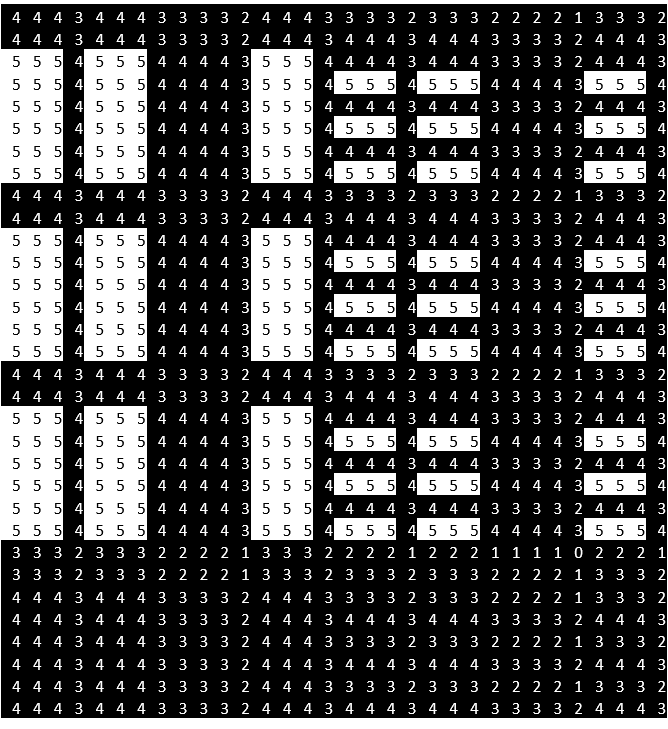
\includegraphics[width=8.0cm]{img/4}\\}
			\only<7>{\centering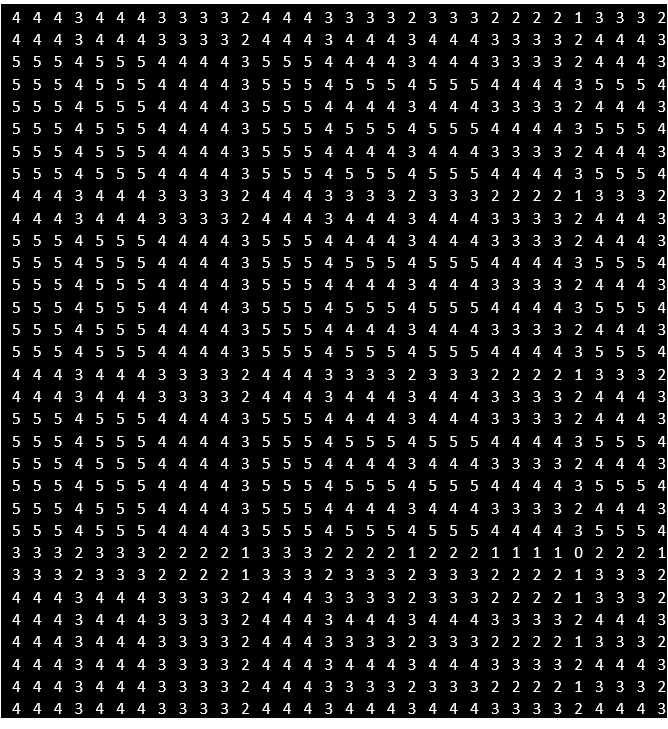
\includegraphics[width=8.0cm]{img/5}\\}
			\end{column}
			\begin{column}{2.0cm}
			\ \vspace*{0.3cm}\\\ \\\ \\\ \\\ \\\ \\\ \\\ \\\ \\
			\ \\\ \\\ \\\ \\\ \\\ \\\ \\\ \\\ 
			$\leftarrow$ ttttt
			\end{column}
			\end{columns}
	\end{frame}

	% \begin{frame}{Speedup technique}{In terms of prefix and suffix}
		% \begin{columns}[t]
		% 	% \begin{column}{0.1\textwidth}\end{column}
		% 	\begin{column}{0.5\textwidth}
		% 	\centering
		% 	\texttt{\color{blue}\Huge acgtacg}\\
		% 	$x$'s {\color{blue}prefix $y$} of length ($l-k$)\\
		% 	determines which patterns\\
		% 	apply to which blocks.\\\ \\

		% 	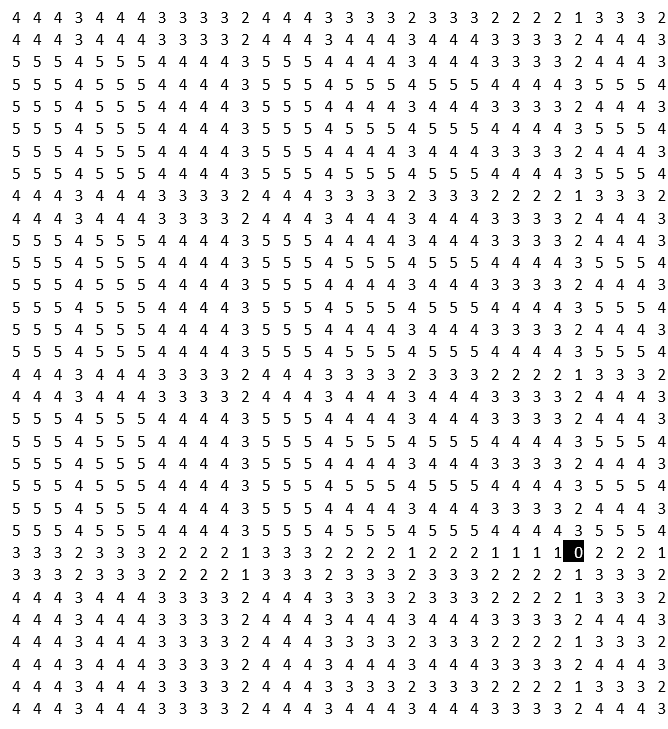
\includegraphics[width=0.25\textwidth]{img/0.png}\ \ 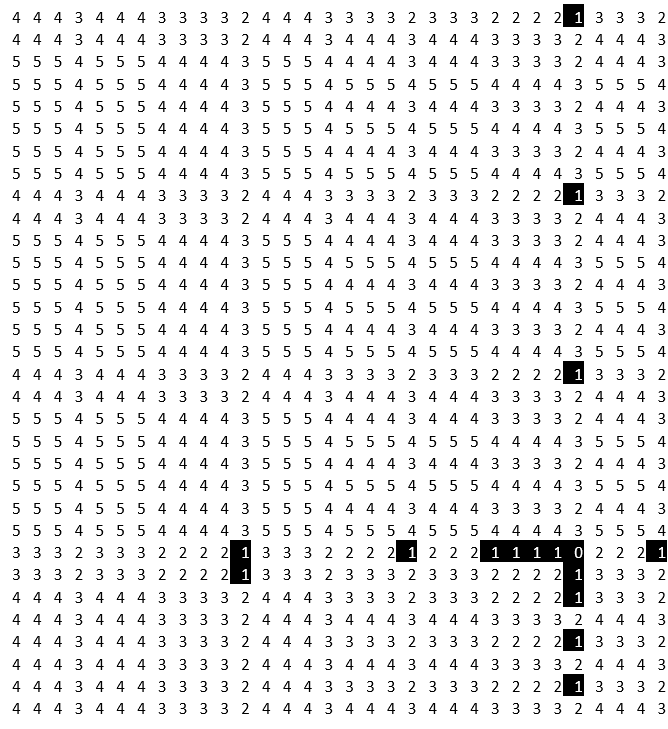
\includegraphics[width=0.25\textwidth]{img/1.png}\\
		% 	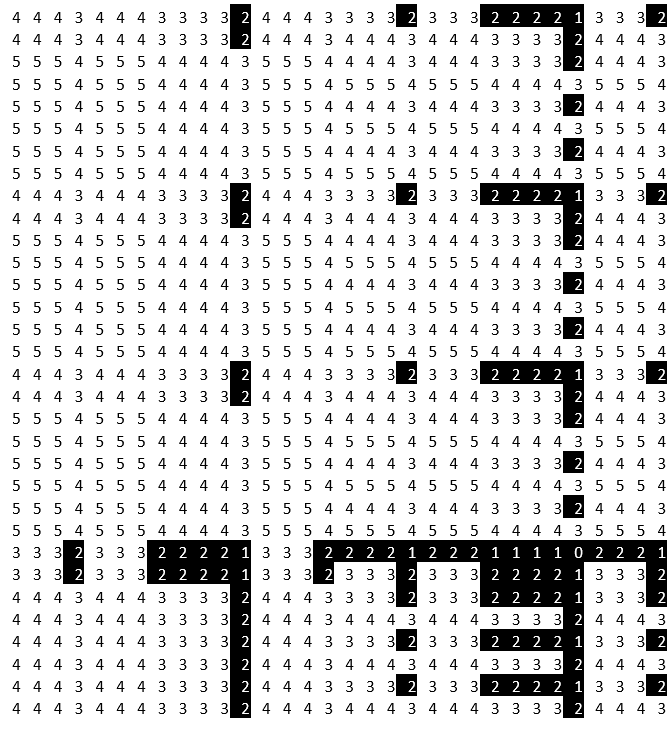
\includegraphics[width=0.25\textwidth]{img/2.png}\ \ 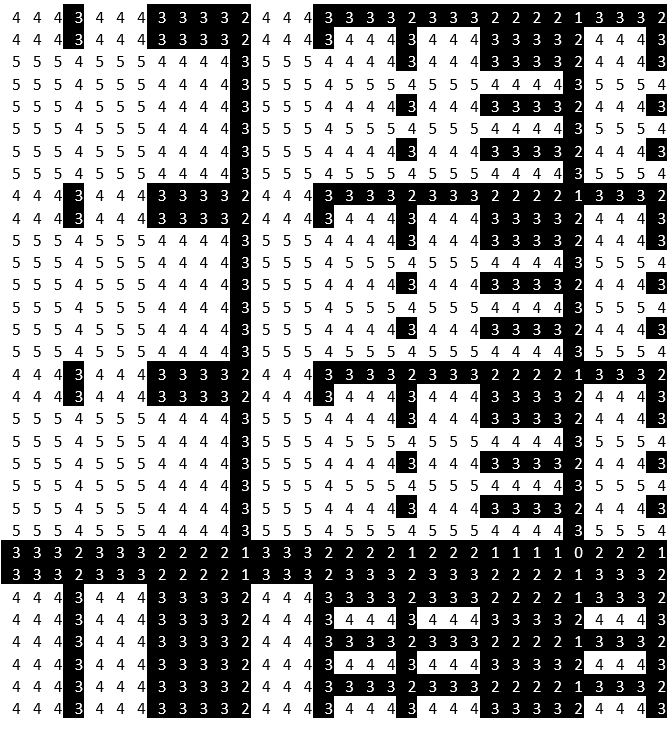
\includegraphics[width=0.25\textwidth]{img/3.png}\\
		% 	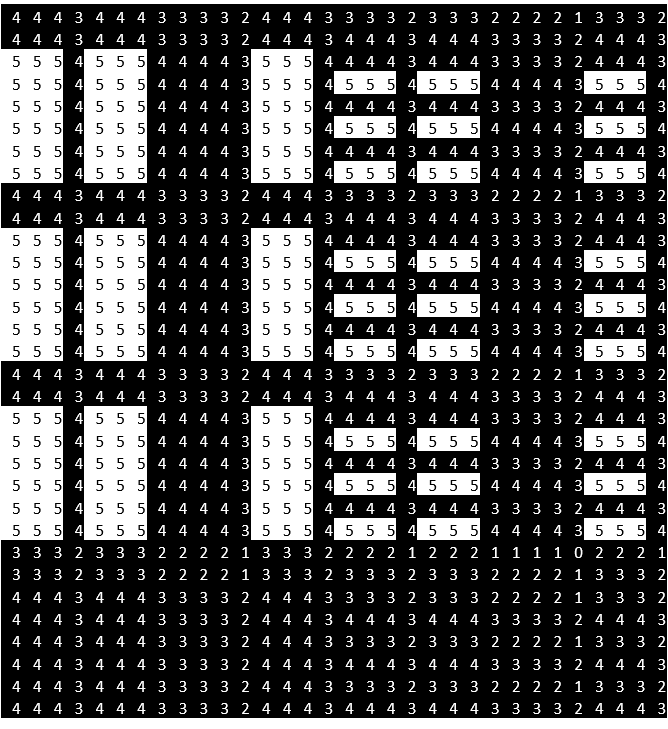
\includegraphics[width=0.25\textwidth]{img/4.png}\ \ 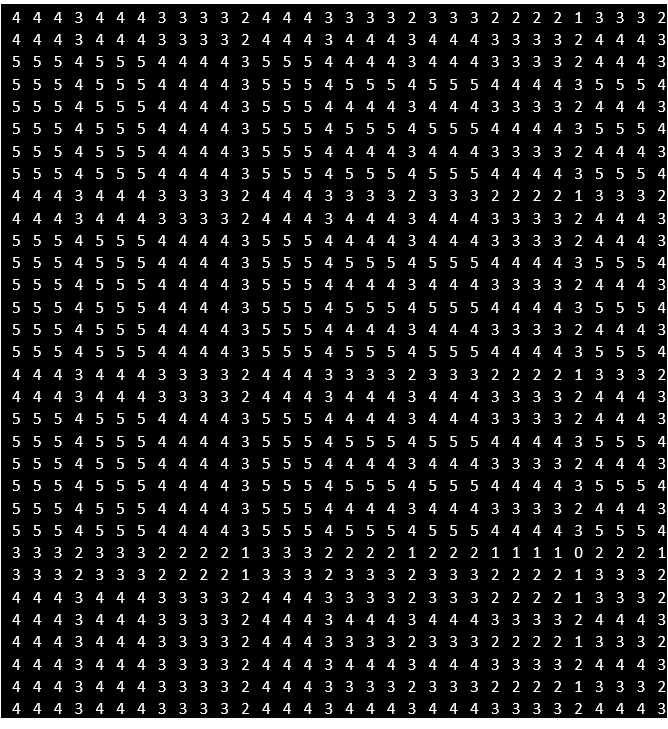
\includegraphics[width=0.25\textwidth]{img/5.png}\\

		% 	\end{column}

		% 	\begin{column}{0.5\textwidth}
		% 	\centering
		% 	\texttt{\color{red}\Huge tacgt}\\
		% 	$x$'s {\color{red}suffix $z$} of length $k$\\
		% 	determines the structure\\
		% 	of the ($k+2$) patterns.\\\ \\
		% 	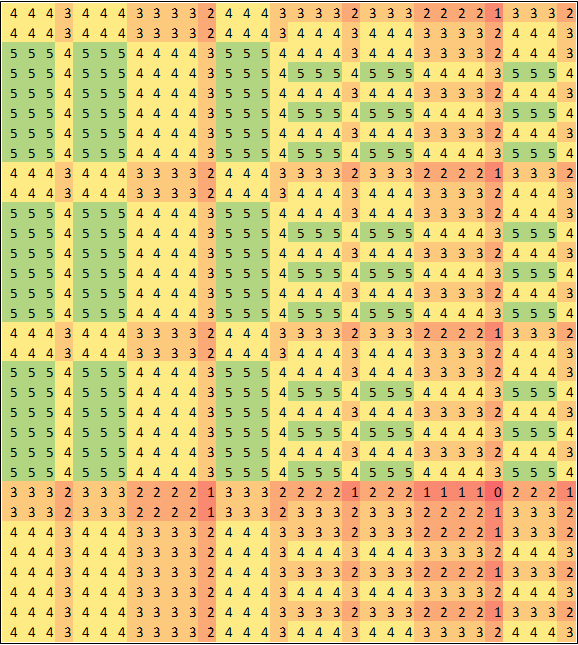
\includegraphics[width=0.75\textwidth]{img/D(tacgt)}

		% 	\end{column}
		% \end{columns}
		% \end{frame}

	% \begin{frame}{Speedup technique}{In terms of prefix and suffix}
		% \begin{itemize}
		% \setbeamercovered{transparent=25}
		% \item<1,2>{\alt<2>{\usebeamercolor[fg]{frametitle}}{} A $4^l$-bit array $N_x$ representing an $l$-mer neighborhood}
		% 	\only<2>{\\The distance between two $l$-mers is the sum of the distances between their {\color{blue} prefixes}
		% 			and between their {\color{red} suffixes}; therefore,\\\ \\
		% 			$
		% 			N_x[\ x'\ ] = \left\{
		% 			\begin{array}{rl}
		% 				1 & \text{if } {\color{blue}d_H(y,y')} + {\color{red}d_H(z,z')} \leq d,\\
		% 				0 & \text{otherwise.}%\text{if } d_{y'} + \mathcal{D}(z)_{z'} > d.
		% 			\end{array} \right.
		% 			\text{ for }x' = y'z'.
		% 			$\\\ \\
		% 			This means we set a bit iff ${\color{red} d_H(z,z')} \leq {\color{blue} d - d_H(y,y')}$.\\\ \\
		% 			% Let $x$ = \texttt{{acgtacg}{tacgt}}, $d$ = 6. \\\ \\
		% 	}
		% \item<1,3>{\alt<3>{\usebeamercolor[fg]{frametitle}}{} can be divided into consecutive $4^k$-bit blocks,}
		% 	\only<3>{\\
		% 	Blocks in $N_x$ for $x$=\texttt{acgtacgtacgt}, $k$=5:
		% 	\footnotesize\\\ \\
		% 		Block 0:\ \ \ \ \ \ \ \ bit flags for 
		% 		\texttt{{\color{blue}aaaaaaa}{\color{red}aaaaa} - {\color{blue}aaaaaaa}{\color{red}ttttt}}\\
		% 		Block 1:\ \ \ \ \ \ \ \ bit flags for 
		% 		\texttt{{\color{blue}aaaaaac}{\color{red}aaaaa} - {\color{blue}aaaaaac}{\color{red}ttttt}}\\
		% 		% Block 2:\ \ \ \ \ \ \ \ bit flags for 
		% 		% \texttt{{\color{blue}aaaaaag}{\color{red}aaaaa} - {\color{blue}aaaaaag}{\color{red}ttttt}}\\
		% 		...\ \ \ \ \ \ \ \ \ \ \ \ \ \ \ \ ...\\
		% 		Block 1,734:\ \ \ bit flags for
		% 		\texttt{{\color{blue}acgtacg}{\color{red}aaaaa} - {\color{blue}acgtacg}{\color{red}ttttt}}\\
		% 		...\ \ \ \ \ \ \ \ \ \ \ \ \ \ \ \ ...\\ 
		% 		Block 16,833: bit flags for 
		% 		\texttt{{\color{blue}ttttttg}{\color{red}aaaaa} - {\color{blue}ttttttg}{\color{red}ttttt}}\\
		% 		Block 16,834: bit flags for 
		% 		\texttt{{\color{blue}ttttttt}{\color{red}aaaaa} - {\color{blue}ttttttt}{\color{red}ttttt}}\\\ \\
		% 	\normalsize The $l$-mers in each block all have the same {\color{blue} prefix}.\\
		% 	Blocks all follow the same sequence of {\color{red}suffixes} (aaaaa - ttttt).\\\ \\
		% 	}
		% \item<1,4>{\alt<4>{\usebeamercolor[fg]{frametitle}}{} and each block will conform to one of ($k + 2$) patterns.}
		% 	\only<4>{\\%A bit is set if $d_H(z,z') \leq d - d_H(y,y')$; \\
		% 	We set a bit iff $\footnotesize{\color{red} d_H(z,z')} \leq {\color{blue} d - d_H(y,y')}$; $\footnotesize 0 \leq {\color{red} d_H(z,z')} \leq k$, therefore there are ($k+2$) ways to set bits in a block:\\\ \\
		% 	\footnotesize
		% 	\begin{columns}[t]
		% 		\begin{column}{0.1\textwidth}\end{column}
		% 		\begin{column}{0.25\textwidth}
		% 			For blocks where:\\
		% 			$\color{blue}d - d_H(y,y')$ $< 0$\\
		% 			$\color{blue}d - d_H(y,y')$ $= 0$\\
		% 			$\color{blue}d - d_H(y,y')$ $= 1$\\
		% 			$\color{blue}d - d_H(y,y')$ $= 2$\\
		% 			...\\
		% 			$\color{blue}d - d_H(y,y')$ $= k$-1\\
		% 			$\color{blue}d - d_H(y,y')$ $= k$\\
		% 		\end{column}
		% 		\begin{column}{0.7\textwidth}
		% 			we set bits for:\\
		% 			no suffixes\\
		% 			{\color{red} suffix $z$} only\\
		% 			suffixes with {\color{red}up to 1 mismatch} with $z$\\
		% 			suffixes with {\color{red}up to 2 mismatches} with $z$\\
		% 			...\\
		% 			suffixes with {\color{red}up to $k$-1 mismatches} with $z$\\
		% 			suffixes with {\color{red}up to $k$ mismatches} with $z$ (all suffixes)\\
		% 		\end{column}
		% 	\end{columns}
			
		% 	}
		% \end{itemize}
		% \end{frame}

	% \begin{frame}{Speedup technique}{Block patterns in the neighborhood of \texttt{acgtacgtacgt}}
		% \centering
		% \begin{columns}
		% 	\footnotesize
		% 	% \begin{column}{0.02\textwidth}\end{column}
		% 	\begin{column}{0.3\textwidth}
		% 		\centering
		% 		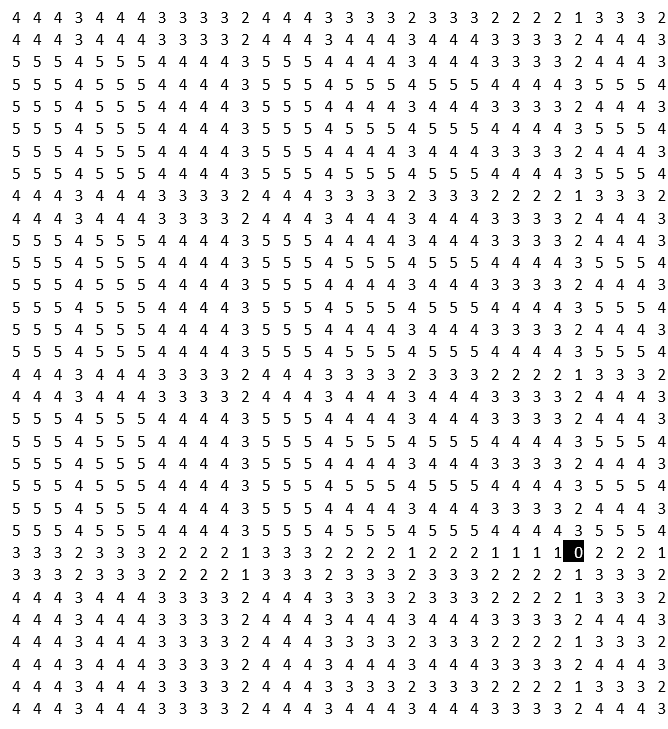
\includegraphics[width=0.9\textwidth]{img/0.png}\\ $\color{blue}d_H(y,prefix) = d$\\\ \\
		% 		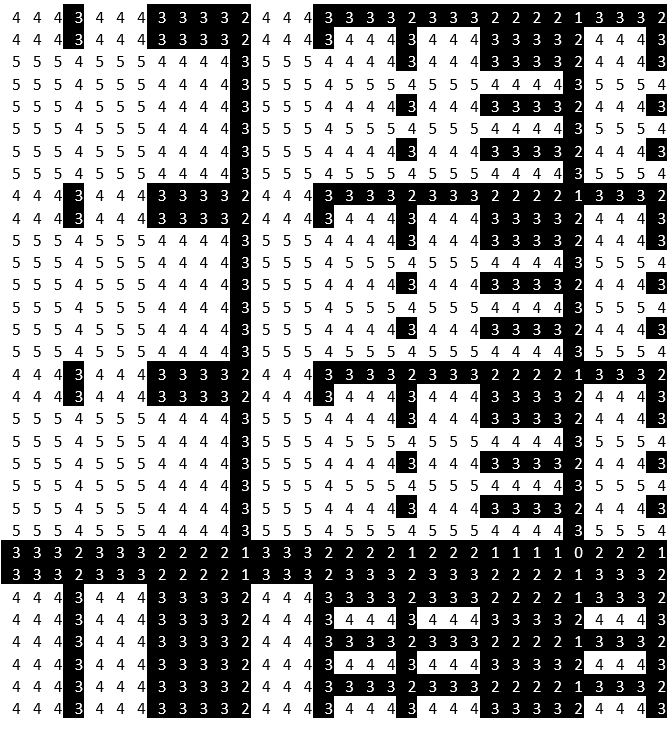
\includegraphics[width=0.9\textwidth]{img/3.png}\\ $\color{blue}d_H(y,prefix) = d-3$\\\ \\
		% 	\end{column}
		% 	\begin{column}{0.3\textwidth}
		% 		\centering
		% 		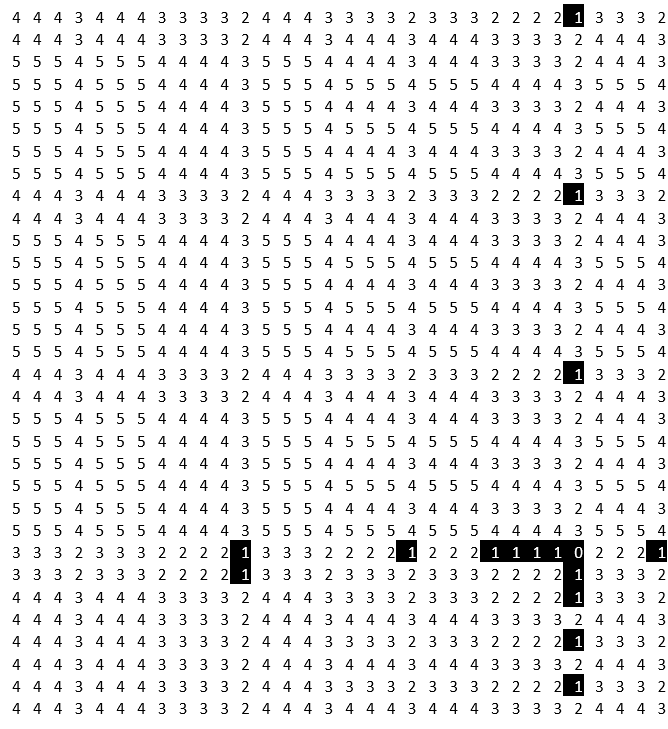
\includegraphics[width=0.9\textwidth]{img/1.png}\\ $\color{blue}d_H(y,prefix) = d-1$\\\ \\
		% 		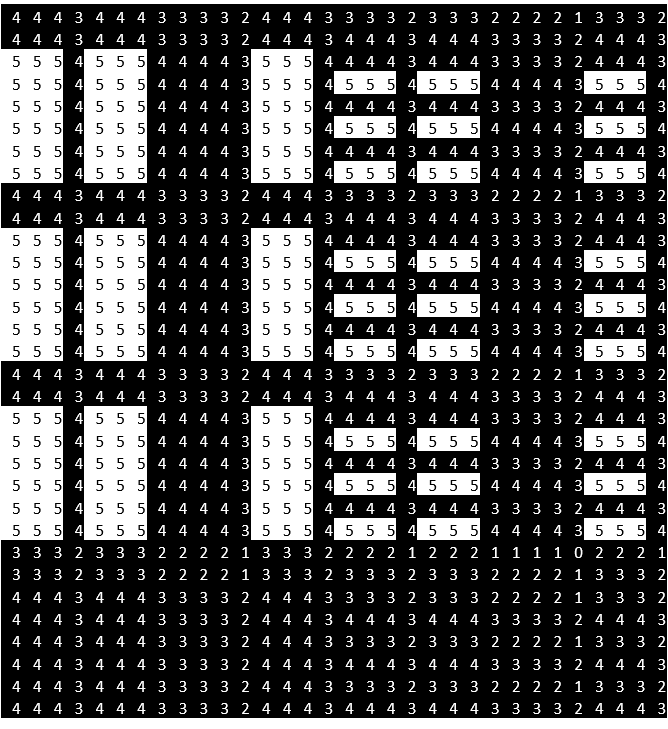
\includegraphics[width=0.9\textwidth]{img/4.png}\\ $\color{blue}d_H(y,prefix) = d-4$\\\ \\
		% 	\end{column}
		% 	\begin{column}{0.3\textwidth}
		% 		\centering
		% 		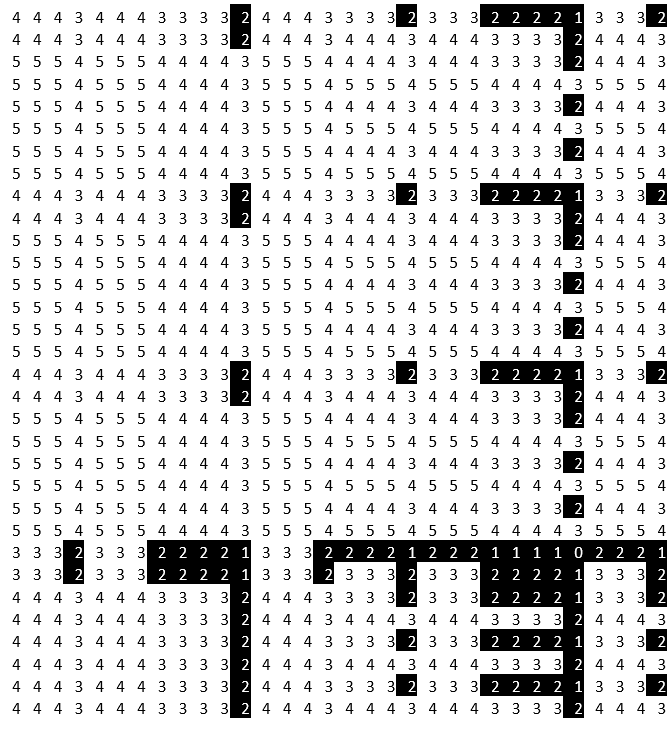
\includegraphics[width=0.9\textwidth]{img/2.png}\\ $\color{blue}d_H(y,prefix) = d-2$\\\ \\
		% 		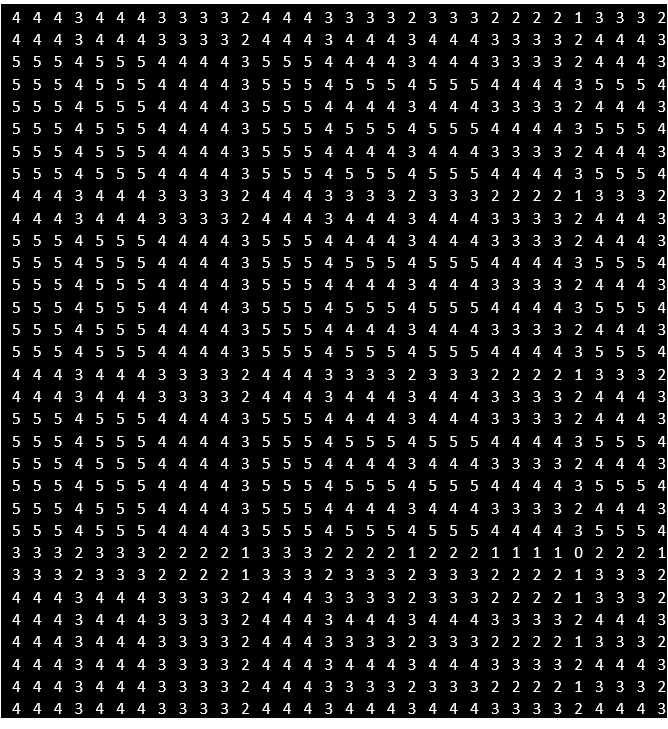
\includegraphics[width=0.9\textwidth]{img/5.png}\\ $\color{blue}d_H(y,prefix) = d-5$\\\ \\
		% 	\end{column}
		% \end{columns}
		% \end{frame}

	\begin{frame}{Speedup technique}{Generate and apply patterns}
		To generate $N_x$ for $x={\color{black}y}{\color{black}z}$, we perform two steps:\\\ \\
		\begin{enumerate}
		\item From {\color{black} $x$}'s suffix $z$, generate $P$, the set of block patterns.\\\ \\
		\begin{columns}
			\begin{column}{0.12\textwidth}\end{column}
			\begin{column}{0.12\textwidth}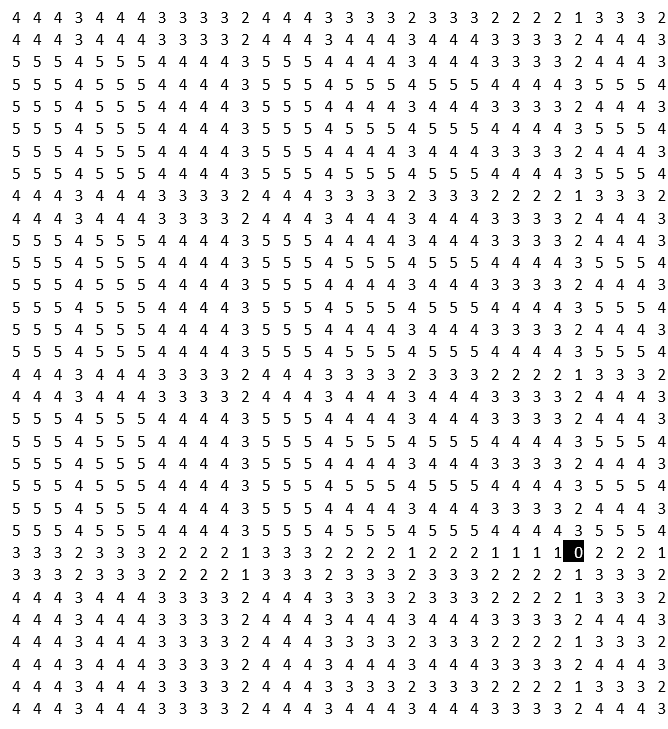
\includegraphics[width=\textwidth]{img/0}\\ \centering $P_0$ \end{column}
			\begin{column}{0.12\textwidth}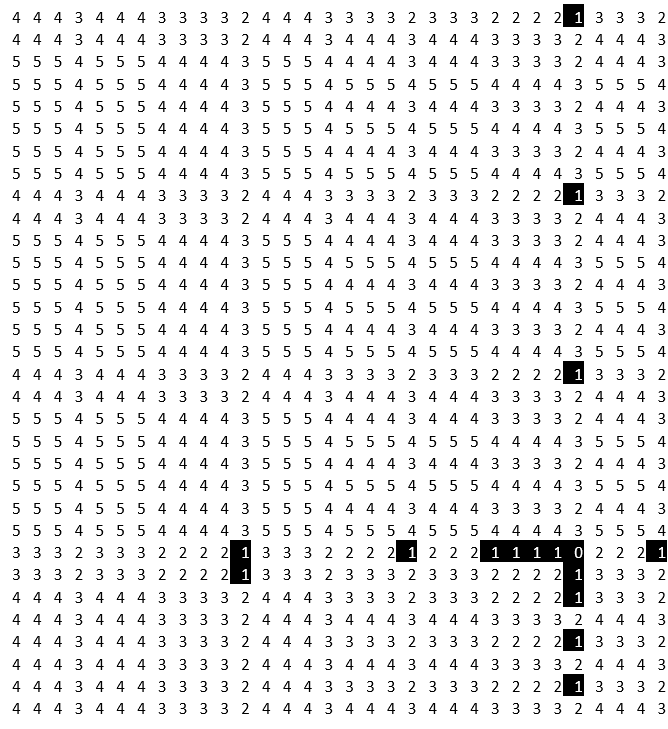
\includegraphics[width=\textwidth]{img/1}\\ \centering $P_1$ \end{column}
			\begin{column}{0.12\textwidth}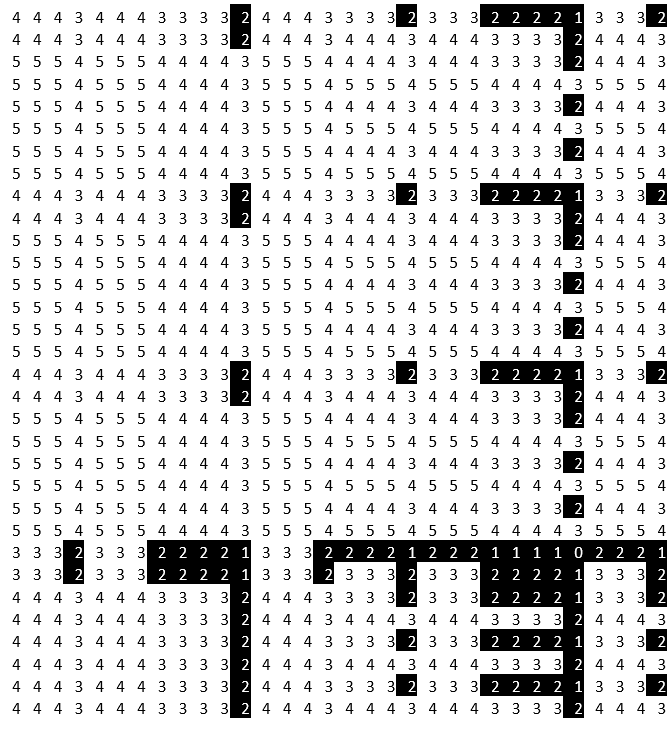
\includegraphics[width=\textwidth]{img/2}\\ \centering $P_2$ \end{column}
			\begin{column}{0.12\textwidth}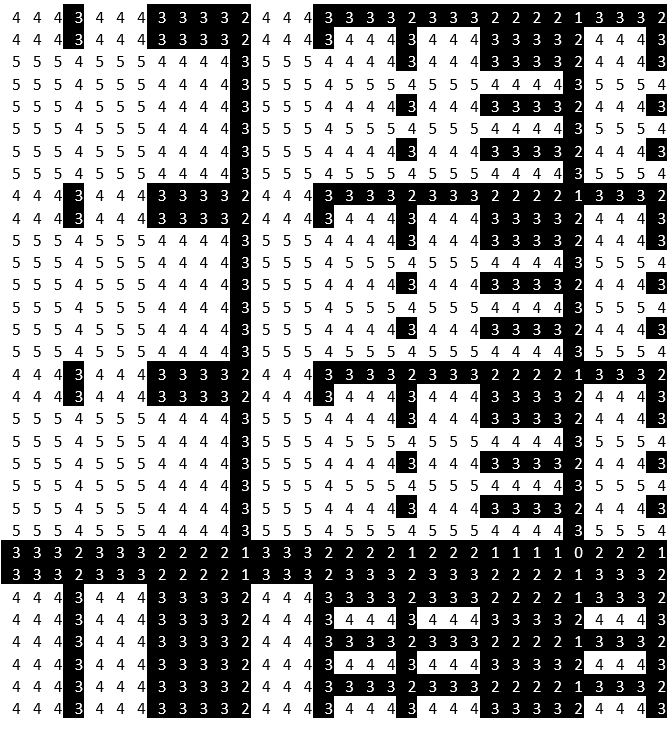
\includegraphics[width=\textwidth]{img/3}\\ \centering $P_3$ \end{column}
			\begin{column}{0.12\textwidth}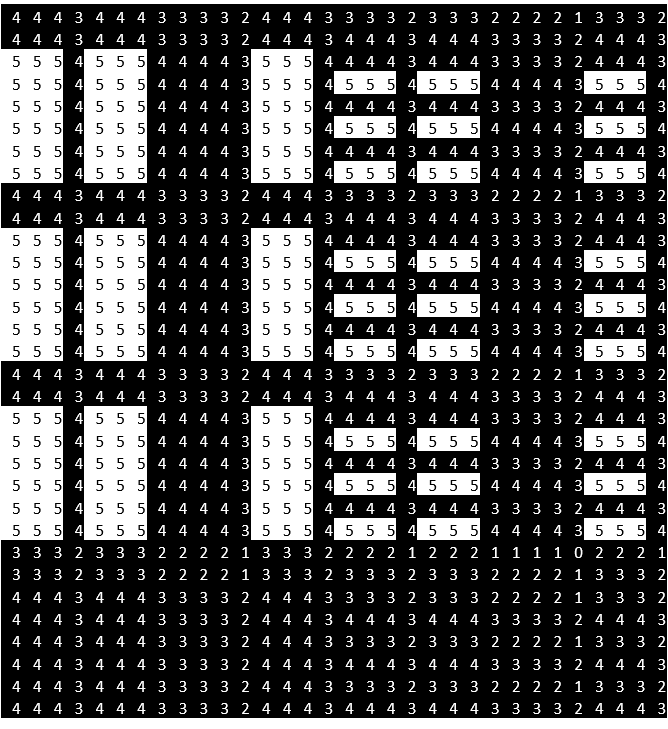
\includegraphics[width=\textwidth]{img/4}\\ \centering $P_4$ \end{column}
			\begin{column}{0.12\textwidth}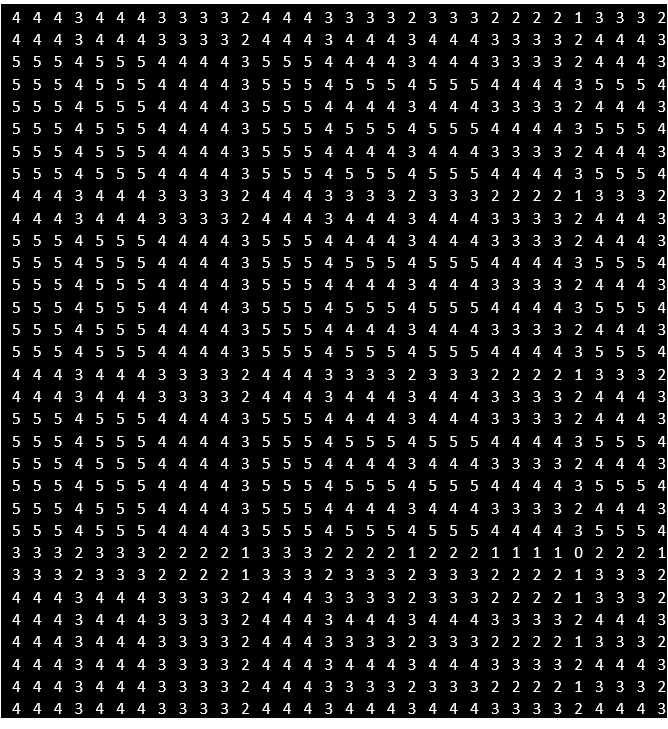
\includegraphics[width=\textwidth]{img/5}\\ \centering $P_5$ \end{column}
			\begin{column}{0.12\textwidth}\end{column}
		\end{columns}\ \\\ \\
		% {\usebeamercolor[fg]{frametitle}Generate the set $\mathcal{P}$} of ($k+2$) block patterns, based on the distribution of Hamming distances from $x$'s {\color{red} suffix $z$} to all possible suffixes $z'$.\\\ \\
		\item From $x$'s prefix $y$, recursively generate each $d$-neighbor $y'$, and apply $P_{(d - d_H(y,y'))}$ to the block whose prefix is $y'$.

		\end{enumerate}
	\end{frame}

\section{Results}
	\subsection{Performance improvement}
	\begin{frame}{Results}{Reduction in recursive neighbor generation} %{Performance improvement with speedup technique}
		{\centering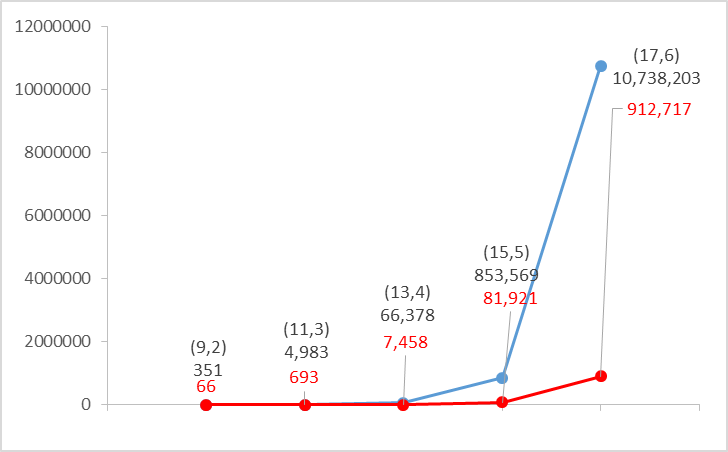
\includegraphics[width=0.8\textwidth]{img/nbrhd_growth_compare.png}\\}
		\begin{itemize}
		\item We still generate $d$-neighbors recursively, but for a shorter sequence $y$, of length $l-k$;
		this graph shows that, for $k$=5, neighborhood size is reduced by a factor of 10.
		\end{itemize}
		% \begin{table}[h] %neighbors_blockmasking
		% 	\footnotesize
		% 	\renewcommand{\arraystretch}{1.3}
		% 	\label{tbl:neighbors_blockmasking}
		% 	\centering
		% 	\begin{tabular}{|c|c|c|c|}
		% 	\hline 
		% 	\bfseries\boldmath $(l,d)$ & \bfseries\boldmath Without speedup & \bfseries\boldmath With speedup, $k$=5 & \bfseries \% reduction\\
		% 	 & $|N(x,d)|$ & $|N(y,d)|$ & \\
		% 	\hline
		% 	 9,2 &         351  &       66 & 81.2\%\\
		% 	11,3 &       4,983  &      693 & 86.1\%\\
		% 	13,4 &      66,378  &    7,458 & 88.8\%\\
		% 	% 14,4 &      91,770  &   12,825 & 86.0\%\\
		% 	15,5 &     853,569  &   81,921 & 90.4\%\\
		% 	% 16,5 &   1,225,092  &  143,979 & 88.2\%\\
		% 	17,6 &  10,738,203  &  912,717 & 91.5\%\\
		% 	\hline\end{tabular}
		% 	\end{table}
		% {\centering \footnotesize Reduction in neighborhood size without vs. with speedup \\}
		\end{frame}

	\begin{frame}{Results}{{\bf EMS-GT \color{blue}without} vs. {\bf\color{red}with} the speedup technique\\} %{Performance improvement with speedup technique}
		% \begin{table}[h] %speedup_blockmasking
		% 	\small
		% 	\renewcommand{\arraystretch}{1.3}
		% 	\label{tbl:speedup_blockmasking}
		% 	\centering
		% 	\begin{tabular}{|c|c|c|c|}
		% 	\hline 
		% 	\bfseries\boldmath $(l,d)$ & \bfseries Without speedup & \bfseries With speedup, $k$=5 & \bfseries \% reduction\\
		% 	% \bfseries & \bfseries procedure & \bfseries\boldmath procedure, $k=5$ & \bfseries\\
		% 	\hline
		% 	 (9,2) &   0.06 s &    0.11 s &     --  \\
		% 	(11,3) &   0.22 s &    0.20 s &    6.7\%\\
		% 	(13,4) &   1.98 s &    1.04 s &   47.5\%\\
		% 	% 14,4 &   3.53 s &    2.55 s &   27.8\%\\
		% 	(15,5) &  25.06 s &   15.51 s &   38.1\%\\
		% 	% 16,5 &  41.63 s &   29.03 s &   30.3\%\\
		% 	(17,6) & 308.61 s &  175.85 s &   43.0\%\\
		% 	\hline\end{tabular}
		% 	\end{table}

		{\centering
		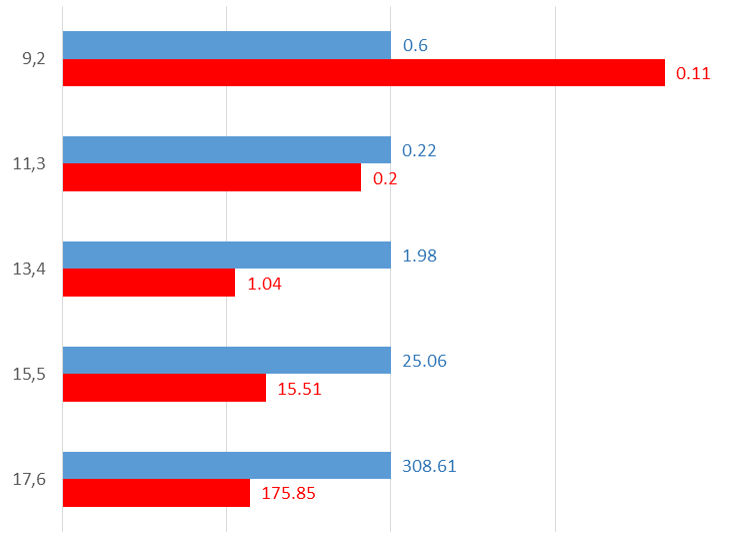
\includegraphics[width=0.8\textwidth]{img/results1.png}\\
		% EMS-GT {\bf\color{blue}without} vs. {\bf\color{red}with} the speedup technique\\
		\footnotesize Runtime in seconds, averaged over 20 synthetic datasets per ($l$,$d$) \\}
		\end{frame}

	\subsection{Performance against PMS8 and qPMS9}
	\begin{frame}{Results}{ {\bf\color{blue}PMS8} vs. {\bf\color{blue}qPMS9} vs. {\bf\color{red}EMS-GT with speedup technique} }%{Performance against PMS8 and qPMS9}
		% \begin{table}[ht] %runtimes
		% 	\small
		% 	\renewcommand{\arraystretch}{1.3}
		% 	\label{tbl:runtimes_v_pms}
		% 	\centering
		% 	\begin{tabular}{|c|c|c|c|c|}
		% 	\hline \bfseries{\boldmath $(l,d)$} & \bfseries PMS8 & \bfseries qPMS9 & \bfseries EMS-GT & \bfseries \% reduction\\
		% 	\hline
		% 	 (9,2) &  0.74 s  &  0.47 s & {\color{blue} 0.11 s} & 76.6\%\\
		% 	(11,3) &  1.58 s  &  1.06 s & {\color{blue} 0.20 s} & 81.1\%\\
		% 	(13,4) &  5.39 s  &  4.52 s & {\color{blue} 1.04 s} & 77.0\%\\
		% 	% 14,4 &  1.29 s  &  1.02 s &      2.55 s\\
		% 	(15,5) & 36.45 s  & 24.63 s & {\color{blue}15.51 s} & 37.0\%\\
		% 	% 16,5 &  4.79 s  &  2.96 s &     29.03 s\\
		% 	(17,6) &  3.91 min & {\color{blue}1.96 min} & {2.93 min} & --\\
		% 	\hline\end{tabular}
		% 	\end{table}

		{\centering 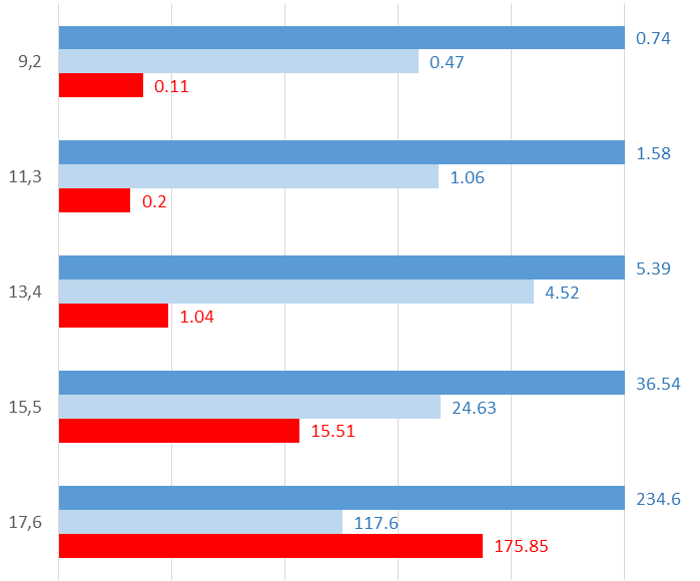
\includegraphics[width=0.8\textwidth]{img/results2.png}\\
		% {\bf\color{blue}PMS8} vs. {\bf\color{blue}qPMS9} vs. {\bf\color{red}EMS-GT with speedup technique}\\
		\footnotesize Runtime in seconds, averaged over 20 synthetic datasets per ($l$,$d$) \\}

		\end{frame}

\section{Conclusions}
	\begin{frame}{Conclusions}
		\begin{itemize}
		\item speedup technique
		\item runtime improvement
		\item comparison with state-of-the-art
		\end{itemize}
		\end{frame}

\end{document}